%%%%%%%%%%%%%%%%%%%%%%%%%%%%%%%%%%%%%%%%%
% BA04 presentation 
% LaTeX Template
% Version 1.0 (14/12/14)
%
% This template has been downloaded from:
% http://www.LaTeXTemplates.com
%
% License:
% CC BY-NC-SA 3.0 (http://creativecommons.org/licenses/by-nc-sa/3.0/)
%
%%%%%%%%%%%%%%%%%%%%%%%%%%%%%%%%%%%%%%%%%

%----------------------------------------------------------------------------------------
%	PACKAGES AND THEMES
%----------------------------------------------------------------------------------------

\documentclass{beamer}
\definecolor{links}{HTML}{2A1B81}
\definecolor{applegreen}{rgb}{0.0, 0.5, 0.0}
\hypersetup{colorlinks,linkcolor=,urlcolor=links}

\mode<presentation> {

% The Beamer class comes with a number of default slide themes
% which change the colors and layouts of slides. Below this is a list
% of all the themes, uncomment each in turn to see what they look like.

%\usetheme{default}
%\usetheme{AnnArbor}
%\usetheme{Antibes}
%\usetheme{Bergen}
%\usetheme{Berkeley}
%\usetheme{Berlin}
%\usetheme{Boadilla}
%\usetheme{CambridgeUS}
%\usetheme{Copenhagen}
%\usetheme{Darmstadt}
%\usetheme{Dresden}
%\usetheme{Frankfurt}
%\usetheme{Goettingen}
%\usetheme{Hannover}
%\usetheme{Ilmenau}
%\usetheme{JuanLesPins}
%\usetheme{Luebeck}
%\usetheme{Madrid}
%\usetheme{Malmoe}
\usetheme{Marburg}
%\usetheme{Montpellier}
%\usetheme{PaloAlto}
%\usetheme{Pittsburgh}
%\usetheme{Rochester}
%\usetheme{Singapore}
%\usetheme{Szeged}
%\usetheme{Warsaw}

% As well as themes, the Beamer class has a number of color themes
% for any slide theme. Uncomment each of these in turn to see how it
% changes the colors of your current slide theme.

%\usecolortheme{albatross}
%\usecolortheme{beaver}
%\usecolortheme{beetle}
%\usecolortheme{crane}
%\usecolortheme{dolphin}
%\usecolortheme{dove}
%\usecolortheme{fly}
%\usecolortheme{lily}
%\usecolortheme{orchid}
%\usecolortheme{rose}
%\usecolortheme{seagull}
%\usecolortheme{seahorse}
%\usecolortheme{whale}
%\usecolortheme{wolverine}

%\setbeamertemplate{footline} % To remove the footer line in all slides uncomment this line
%\setbeamertemplate{footline}[page number] % To replace the footer line in all slides with a simple slide count uncomment this line

\setbeamertemplate{navigation symbols}{} % To remove the navigation symbols from the bottom of all slides uncomment this line
}

\usepackage{graphicx} % Allows including images
\usepackage{booktabs} % Allows the use of \toprule, \midrule and \bottomrule in tables
\usepackage[english]{babel}
\usepackage[utf8x]{inputenc}

%----------------------------------------------------------------------------------------
%	TITLE PAGE
%----------------------------------------------------------------------------------------

\title[Deep Learning: A Bayesian Perspective]{Deep Learning: A Bayesian Perspective} % The short title appears at the bottom of every slide, the full title is only on the title page


\author{
E. Benhamou\\
} % Your name

\institute[Université Dauphine] % Your institution as it will appear on the bottom of every slide, may be shorthand to save space
{
Article Reading for Bayesian Nonparametrics\\
Julyan Arbel's course \\
M2 MASH \\
Université Paris Dauphine % Your institution for the title page
}
\date{16 March 2018} % Date, can be changed to a custom date

\begin{document}

\begin{frame}
\titlepage % Print the title page as the first slide
\end{frame}

\begin{frame}
\frametitle{Summary} % Table of contents slide, comment this block out to remove it
\tableofcontents % Throughout your presentation, if you choose to use \section{} and \subsection{} commands, these will automatically be printed on this slide as an overview of your presentation
\end{frame}

%----------------------------------------------------------------------------------------
%	PRESENTATION SLIDES
%----------------------------------------------------------------------------------------

%---------------------------------------------------------------------
%------------------------------------------------
\section{Primer on deep learning} 
\begin{frame}
\frametitle{Primer on deep learning}
\begin{itemize}
\item Deep learning (DL) uses hierarchical abstract layers of latent
variables to perform pattern matching and prediction.
\item It is designed for massive data sets with many high dimensional input variables
\item It is theoretically still not very well understood. They are connections with Bayesian Non Parametric that we review here thanks to \cite{Polson 2017}
\end{itemize}
\end{frame}
%------------------------------------------------

%------------------------------------------------
\subsection{A few facts} 
\begin{frame}
\frametitle{Primer on deep learning}
\framesubtitle{A few facts}
\begin{itemize}
\item DL has existed for more than 50 years (\cite{Rosenblatt 1958}  Perceptron). It was perceived as complex and not very powerful for decades.
\item DL made breakthrough only in the last 5 years. MNIST recognition \cite{Lecun 2013}. 3 researchers have emerged as the main figures
\cite{Yoshua Lecun Hilton 2015}
\end{itemize}
DL is used in many fields:
\begin{itemize}
\item content filtering, 
\item image and face recognition, medical image analysis, neuroscience
\item self-driving cars, robot perception and control, 
\item speech recognition, natural language understanding and translation.
\end{itemize}
\end{frame}
%------------------------------------------------

%------------------------------------------------
\begin{frame}
Deep learning is designed for massive data sets with many high dimensional input variables
\begin{itemize}
\item Google’s translation algorithm \cite{Sutskever et al. 2014} uses $\sim$ 1-2 billion parameters
and very large dictionaries
\item Baidu deployed speech recognition systems \cite{Amodei et al. 2016} with a model over 100 million parameters, 11 layers and almost 12 thousand hours of training.
\end{itemize}
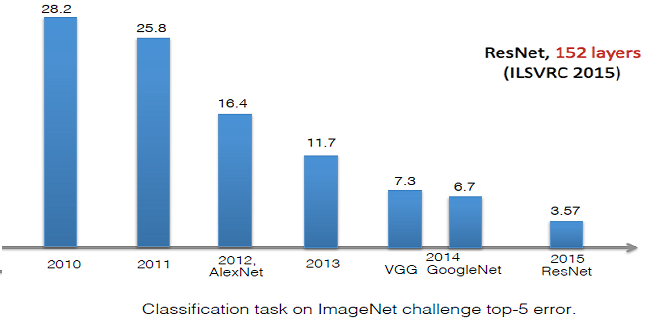
\includegraphics[width=0.9\textwidth]{images/deeplearning_evolution.PNG}
\end{frame}
%------------------------------------------------

%------------------------------------------------
\subsection{Framework}
\begin{frame}
\frametitle{Primer on deep learning}
\framesubtitle{Framework}
There exists many different architectures for deep learning networks.
\begin{center}
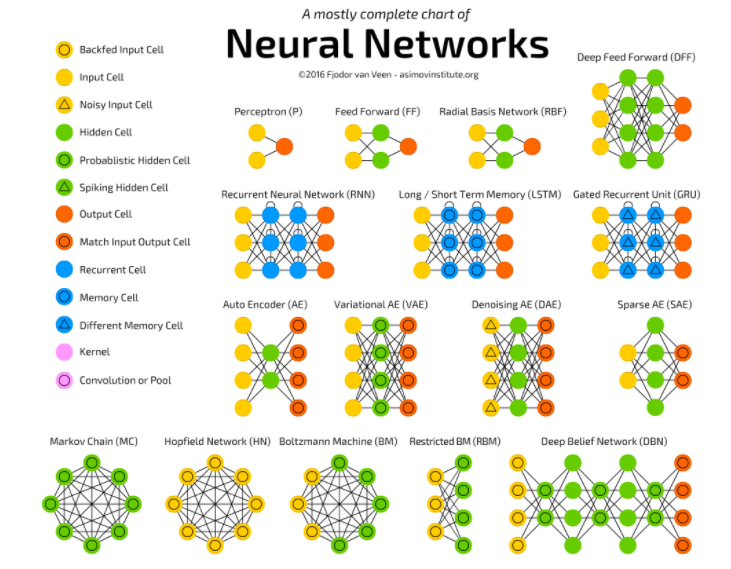
\includegraphics[width=0.45\textwidth]{images/deepnetworks_architecture_1.PNG}
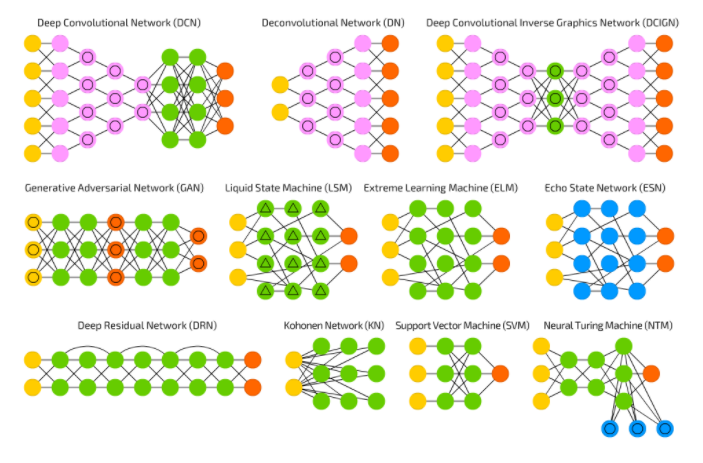
\includegraphics[width=0.45\textwidth]{images/deepnetworks_architecture_2.PNG} 
\end{center}
\end{frame}
\begin{frame}
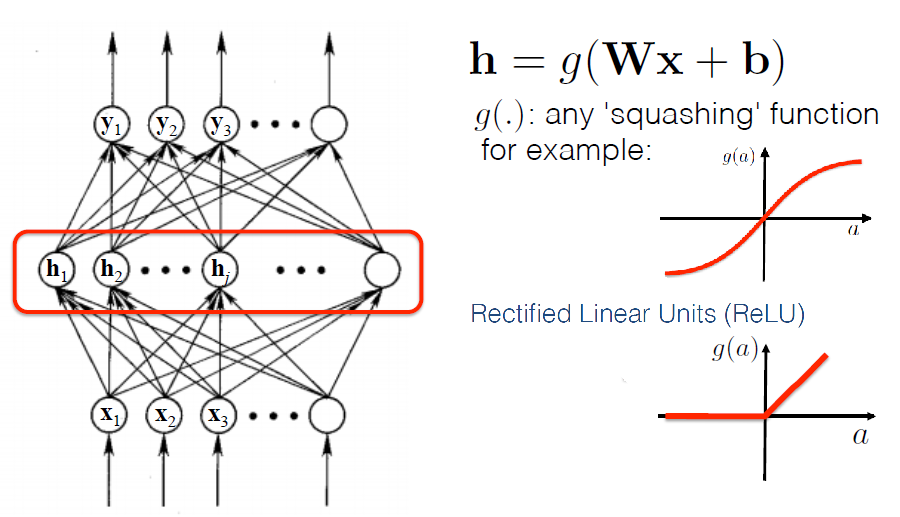
\includegraphics[width=0.9\textwidth]{images/deep_network.PNG}
\end{frame}

\begin{frame}
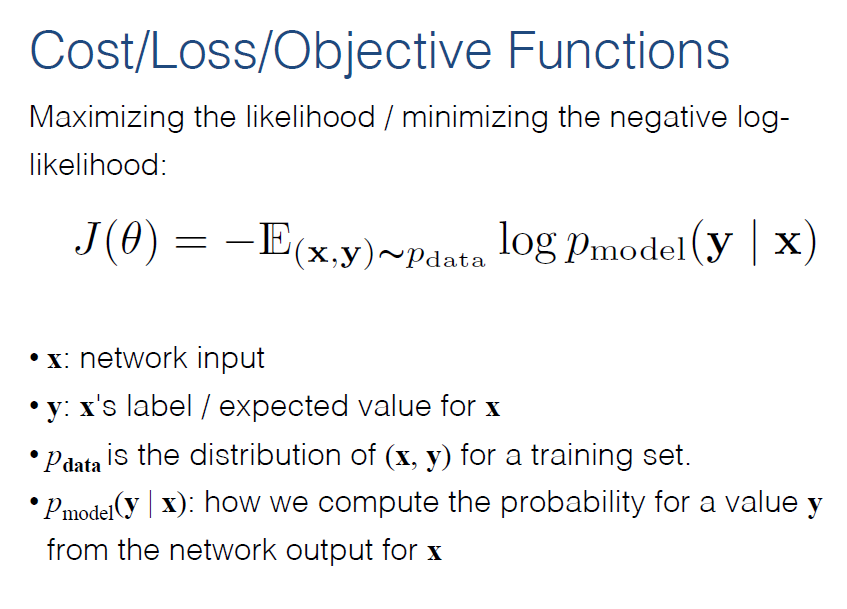
\includegraphics[width=0.9\textwidth]{images/archi_4.PNG} 
\end{frame}
%------------------------------------------------

%---------------------------------------------------------------------
\section{Algorithmic issues}
\subsection{Stochastic Gradient Descent}
%------------------------------------------------
\begin{frame}
\frametitle{Algorithmic issues}
\framesubtitle{Stochastic Gradient Descent}
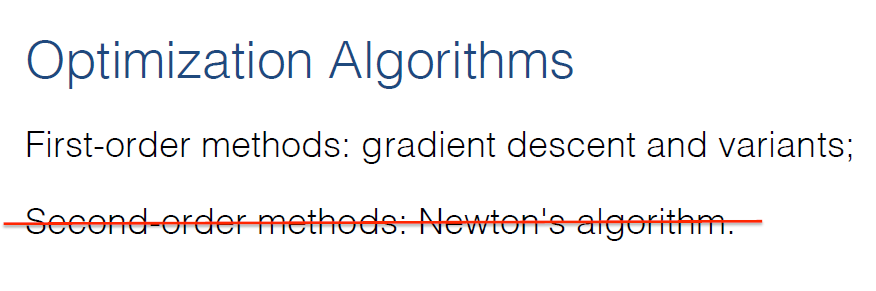
\includegraphics[width=0.9\textwidth]{images/optim_2.PNG} \\
\end{frame}
\begin{frame}
We could think of local minimum problem but reality is the following:
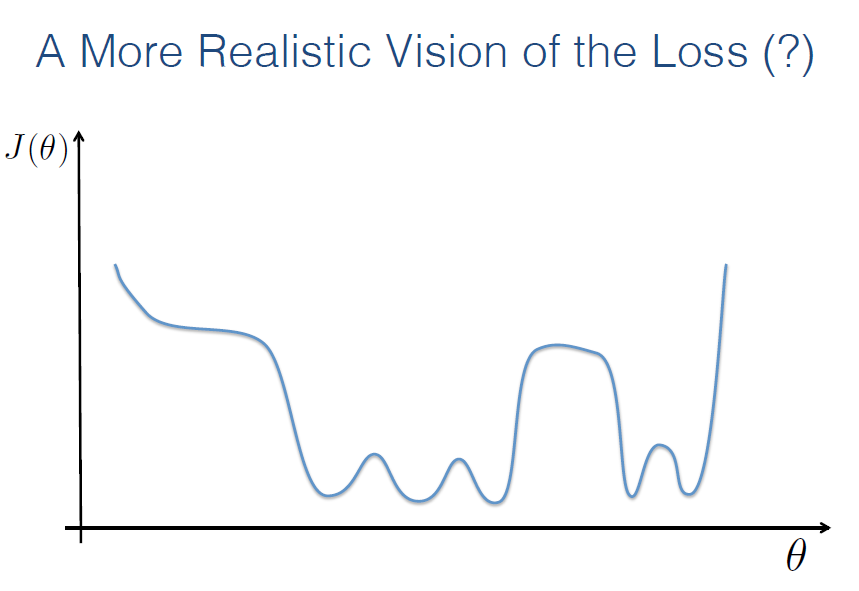
\includegraphics[width=0.9\textwidth]{images/optim_4.PNG} \\
\end{frame}

\subsection{Backprop}
\begin{frame}
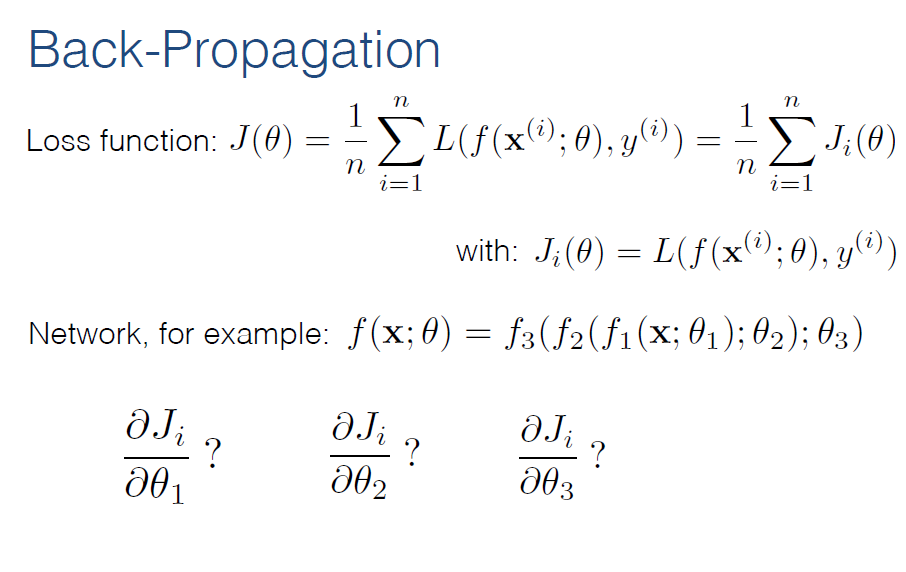
\includegraphics[width=0.9\textwidth]{images/backprop_1.PNG} 
\end{frame}
\begin{frame}
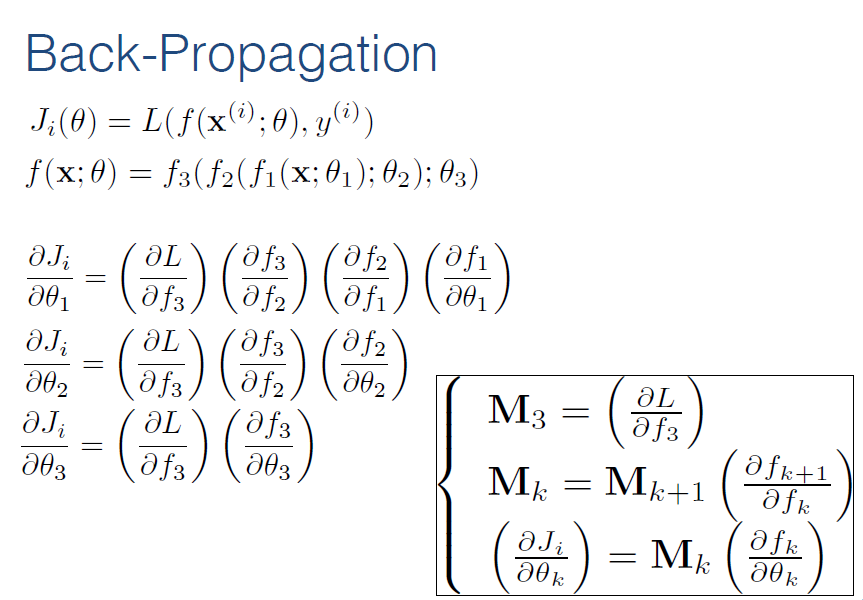
\includegraphics[width=0.9\textwidth]{images/backprop_3.PNG} 
\end{frame}
%------------------------------------------------

\subsection{Dropout}
%------------------------------------------------
\begin{frame}
\frametitle{Algorithmic issues}
\framesubtitle{Dropout}
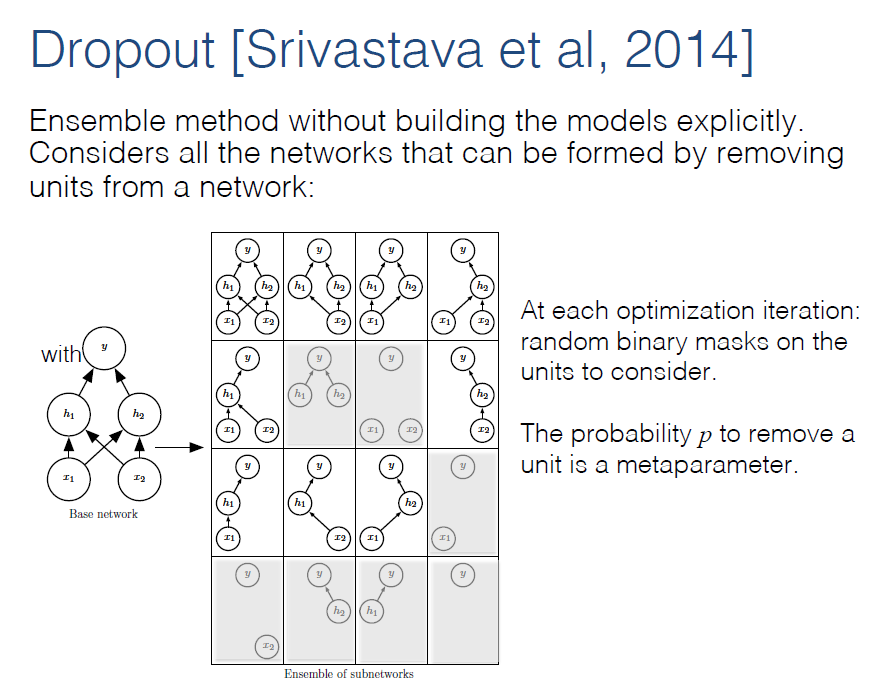
\includegraphics[width=0.9\textwidth]{images/drop_out_1.PNG} \\
Dropout is exact for linear classification but we still do not know how to prove it for more complex networks
\end{frame}
%------------------------------------------------
\begin{frame}
\frametitle{Dropout is efficient (see Leonardo Araujo dos Santos)}
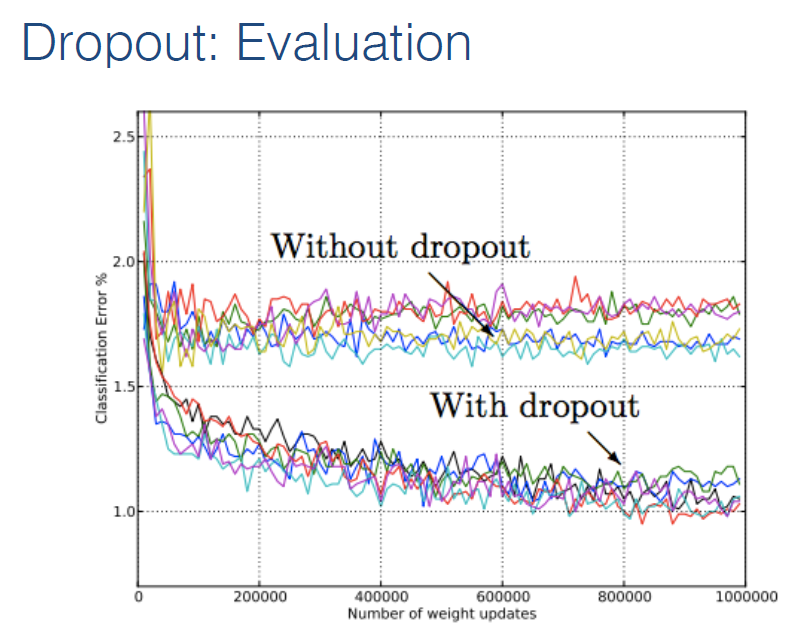
\includegraphics[width=0.9\textwidth]{images/drop_out_6.PNG} \\
It can be shown that dropout training is identical to approximate
inference in Bayesian modeling  \cite{Gal 2016}
\end{frame}
\begin{frame}
Dropout can be seen as a Bayes ridge regression
\\
The problem is 
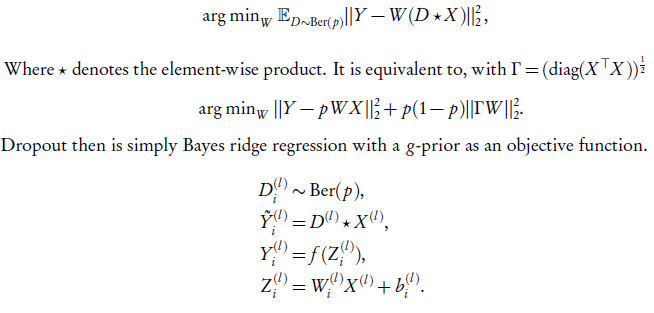
\includegraphics[width=0.9\textwidth]{images/drop_out_7.PNG} \\
\end{frame}
%------------------------------------------------

%---------------------------------------------------------------------
\section{Application: Airbnb challenge}
\subsection{Challenge presentation}
%------------------------------------------------
\begin{frame}
\frametitle{Application: Airbnb challenge}
\framesubtitle{Challenge presentation}
We try to reproduce some results of the article. This concerns the Airbnb Kaggle competition, offered in 2014.
The full link is here: 
\href{https://www.kaggle.com/c/airbnb-recruiting-new-user-bookings}{Airbnb kaggle}
\\
We present here the main points:
\begin{itemize}
\item goal: predict in which country a new user will make his or her first booking
\item database resctricted to 10 countries + other + NDF
\item data consists of 2 tables: attributes of each of the users, data about sessions 
\item  represent 213,451 users and 1,056,7737 individual sessions
\end{itemize}
\end{frame}
%------------------------------------------------

%------------------------------------------------
\begin{frame}
Full code is available in 
 \href{https://github.com/ericbenhamou/BayesianNonParametric}{github}
\\
Using barplot, we can give an intuition about the data
\includegraphics[width=0.9\textwidth]{images/data_challenge_1.PNG} 
\end{frame}
%------------------------------------------------

%------------------------------------------------
\begin{frame}
\includegraphics[width=0.9\textwidth]{images/data_challenge_2.PNG} 
\end{frame}
%------------------------------------------------

%------------------------------------------------
\begin{frame}
Building a deep net in R is straightforward with the h2o package
It works as follows: \\
\bigskip

{\color{applegreen}  \#\# load library } \\
{\color{blue} library}(h2o) \\
h2o.init(nthreads = -1, max\_mem\_size="2G") \\
{\color{applegreen}  \#\# clean slate (just in case cluster was running) } \\
h2o.removeAll() \\
{\color{applegreen}  \#\# create h2o dataframe } \\
train\_users.hex = as.h2o(train\_users[1:10000,]) 

{\color{applegreen}  \#\# create train and test sets} \\
splits = h2o.splitFrame( \\
\hspace{0.5cm}  train\_users.hex,    c({\color{blue} 0.7},{\color{blue} 0.3}), \\
\hspace{0.5cm}  seed = {\color{blue} 1234})   
\end{frame}
%------------------------------------------------

%------------------------------------------------
\begin{frame}
\frametitle{Code: continued...}
{\color{applegreen}  \#\# assign to variable train and test } \\
train = h2o.assign (splits[[ {\color{blue} 1}]], "train.hex") \\
test  = h2o.assign (splits[[{\color{blue}  2}]], "test.hex")     \\
dl\_model = h2o.deeplearning(  \\
\hspace{0.5cm}    x = {\color{blue} 1} {\color{blue} 15},  \\
\hspace{0.5cm}    y = {\color{blue} 16},  \\
\hspace{0.5cm}    training\_frame = train,  \\
\hspace{0.5cm}    activation = "RectifierWithDropout", \\
\hspace{0.5cm}    hidden = c({\color{blue} 50}), \\
\hspace{0.5cm}    epochs = {\color{blue} 20}, \\
\hspace{0.5cm}    loss = "CrossEntropy", \\
\hspace{0.5cm}    adaptive\_rate = FALSE, \\
\hspace{0.5cm}    rate ={\color{blue} .001}, \\
\hspace{0.5cm}    input\_dropout\_ratio = {\color{blue} 0.1}, \\
\hspace{0.5cm}    hidden\_dropout\_ratios = c({\color{blue} .2}) \\
)
\end{frame}

\begin{frame}
\frametitle{Code: continued...}
{\color{applegreen}  \#\# display summary } \\
summary(dl\_model ) \\
{\color{applegreen}  \#\# validation metrics (confusion matrix)} \\
dl\_model@model\$validation\_metrics     
{\color{applegreen}  \#\# just accuracy } \\
h2o.hit\_ratio\_table(dl\_model ,valid = T)[1,2] \\
\end{frame}


\subsection{Results}
%------------------------------------------------
\begin{frame}
\frametitle{Application: Airbnb challenge}
\framesubtitle{Results}
We managed to get a hit ratio of 0.8252093 compared to the paper of 0.8351
\includegraphics[width=0.9\textwidth]{images/result1.PNG} 
\end{frame}
%------------------------------------------------



%------------------------------------------------
\section{Conclusion}
\begin{frame}
\frametitle{Conclusion}
This paper is quite general and presents the foundation of the usage of Bayesian tools to assist in training deep architecture.
There are many possible extension to Bayesian for deep network:
\begin{itemize}
\item viewing deep learning as a Gaussian Process and doing exact Bayesian inference via posterior
\item using Monte Carlo Markov Chain
\end{itemize}
\end{frame}
%------------------------------------------------



%------------------------------------------------
\begin{frame}
\frametitle{References}
\footnotesize{
\begin{thebibliography}{99} 
% Beamer does not support BibTeX so references must be inserted manually as below
\bibitem[Polson 2017]{Polson 2017} Polson N., V. Sokolov (2017)
\newblock Deep Learning: A Bayesian Perspective
\newblock \emph{arXiv} \href{https://arxiv.org/pdf/1706.00473}{arXiv:1706.00473v4}

\bibitem[Rosenblatt 1958]{Rosenblatt 1958} Rosenblatt, F. (1958)
\newblock The Perceptron: A Probabilistic Model For Information Storage And Organization In The Brain
\newblock \emph{Psychological Review. 65 (6): 386–408} \href{http://citeseerx.ist.psu.edu/viewdoc/download?doi=10.1.1.335.3398&rep=rep1&type=pdf}{citeseerx}

\bibitem[Lecun 2013]{Lecun 2013} LeCun Y., Farabet C., Couprie C., Najman L. (2013)
\newblock Learning Hierarchical Features for Scene Labeling, 
\newblock IEEE Transactions on Pattern Analysis and Machine Intelligence, August 2013

\bibitem[Lecun MNIST 2013]{Lecun MNIST 2013} LeCun, Y.; Corinna C.; C. J.C. Burges (2013)
\newblock MNIST handwritten digit database, 
\newblock \href{http://yann.lecun.com/exdb/mnist}{Download link}

\end{thebibliography}
}
\end{frame}
%------------------------------------------------

%------------------------------------------------
\begin{frame}
\frametitle{References}
\footnotesize{
\begin{thebibliography}{99} 
\bibitem[Yoshua Lecun Hilton 2015]{Yoshua Lecun Hilton 2015} Bengio, Yoshua, LeCun, Yann, Hinton Geoffrey (2015)
\newblock Deep Learning
\newblock \emph{Nature}.521: 436–444 (2015)

\bibitem[Sutskever et al. 2014]{Sutskever et al. 2014} Sutskever I., O. Vinyals, and Quoc V Le (2014)
\newblock Sequence to sequence learning with neural networks.
\newblock In Advances in neural information processing systems, pages 3104–3112, 2014. 2

\bibitem[Amodei et al. 2016]{Amodei et al. 2016}Amodei D., Sundaram Ananthanarayanan, Rishita Anubhai, Jingliang Bai, Eric Battenberg, Carl Case, Jared Casper, Bryan Catanzaro, Qiang Cheng, Guoliang Chen, et al (2016)
\newblock Deep speech 2: End-to-end speech recognition in english and mandarin
\newblock In International Conference on Machine Learning, pages 173–182, (2016)

\bibitem[Gal 2016]{Gal 2016} Y Gal, Z Ghahramani (2016) 
\newblock A Theoretically Grounded Application of Dropout in
\newblock Recurrent Neural Networks”, NIPS (2016)


\end{thebibliography}
}
\end{frame}
%------------------------------------------------

%------------------------------------------------
\begin{frame}
\Huge{\centerline{Questions?}}
\end{frame}

\end{document}